\begin{center}
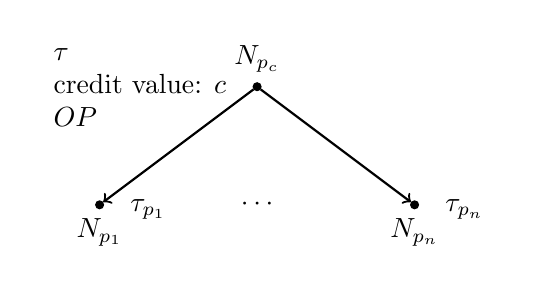
\begin{tikzpicture}[yscale=-1,
place/.style={circle,draw=black, fill=black, inner sep=0pt, 
              minimum size=1mm}]

  \node[place] (1st) at (2, 0) [label=above: $N_{p_c}$,
                                label=left: 
             \begin{tabular}{l}
               $\tau$\\
               credit value: $c$\\
               $OP$\\
             \end{tabular}
] {};
	\node[place] (2nd) at (0, 1.5) [label=below: $N_{p_1}$,
							  label=right: 
             \begin{tabular}{l}
            $\tau_{p_1}$\\
             \end{tabular}
	] {};
        \node[place] (3rd) at (4, 1.5) [label=below: $N_{p_n}$,
        							label=right: 
             \begin{tabular}{l}
             $\tau_{p_n}$ \\
             \end{tabular}        
        ] {}; 
	
	\node (dots) at (2,1.5) {$\cdots$};
	
	\draw[->, thick] (1st) -- (2nd);
	\draw[->, thick] (1st) -- (3rd);
        

\end{tikzpicture}
\end{center}   